\part{Nuclear data}\label{part:nd}

The method touches nuclear data in three places: the CE cross sections that attenuate backward
paths and flights, the production kernels whose densities the evaluators compute, and the collision
routines the sampler route and the flights call. This part starts from the physics of individual
reactions, follows them into the evaluated files and OpenMC's library, shows how they shape the
spectra of a real lattice, and ends with what each reaction means for this method.

\section{Reactions and cross sections}\label{sec:nd:reactions}

\subsection{What a cross section is}

A \textbf{microscopic cross section} $\sigma_x(E)$ is the effective area a nucleus presents to a
neutron of energy $E$ for reaction $x$; its unit is the barn ($10^{-24}$ cm$^2$). The probability of
reaction $x$ per unit path in a material with atom densities $N_i$ is the macroscopic cross section
$\Sigma_x=\sum_iN_i\sigma_{x,i}$ (cm$^{-1}$). The total cross section is the sum over all reactions;
the mean free path is $1/\Sigma_t$. Reactions are identified by ENDF \textbf{MT} numbers: 1 total, 2
elastic, 4 inelastic (sum of 51--91), 16 $(n,2n)$, 18 fission, 51--90 inelastic to discrete levels,
91 inelastic continuum, 102 radiative capture $(n,\gamma)$, 103--107 charged-particle emission.

\subsection{The reactions that matter for neutron transport}

\begin{itemize}
\item \textbf{Elastic scattering} (MT 2) conserves kinetic energy in the centre-of-mass frame; the
  neutron loses energy to the recoiling nucleus. It dominates in moderators and at most energies in
  fuel. It has a potential part (hard-sphere, smooth) and resonance parts.
\item \textbf{Inelastic scattering} (MT 51--91) leaves the nucleus excited. To a discrete level
  (MT 51--90) the Q-value $-Q$ is fixed and the kinematics are two-body; above the highest resolved
  level the continuum (MT 91) is described statistically. Thresholds lie near $|Q|(A+1)/A$; for U-238
  the first level is at 45 keV.
\item \textbf{$(n,xn)$} reactions emit several neutrons; the yield multiplies the production.
\item \textbf{Fission} (MT 18, or partial MT 19--21, 38 for first, second, third and fourth
  chance) emits on average $\bar\nu(E)$ neutrons, prompt and delayed, with an energy spectrum $\chi$
  peaked near 1 MeV.
\item \textbf{Capture} (MT 102) removes the neutron; it matters through $\Sigma_t$ and self-shielding.
\end{itemize}

\begin{figure}[t]\centering
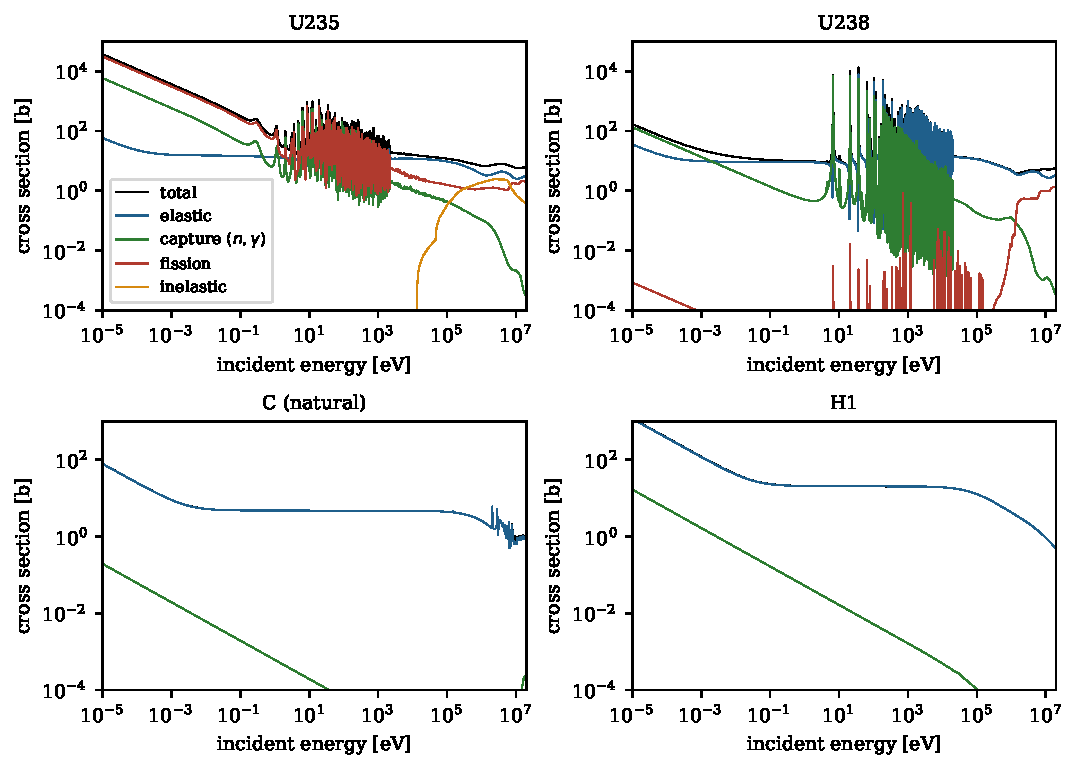
\includegraphics[width=\textwidth]{figures/nd_cross_sections.pdf}
\caption{Cross sections at 294 K from the library used here. U-235: the $1/v$ fission and capture at
low energy, the resolved resonances from 1 eV to 2.25 keV, and smooth fast data. U-238: giant capture
resonances (6.67, 20.9, 36.7 eV, \dots), the inelastic threshold at 45 keV and the fission threshold
near 1 MeV. Carbon: nearly constant elastic scattering up to MeV, then resonances. Hydrogen: elastic
only (plus a small capture), flat to 10 keV.}\label{fig:nd:xs}
\end{figure}

\subsection{Energy ranges}

The data of a heavy nuclide fall into four ranges (Figure~\ref{fig:nd:xs}): the \emph{thermal} range
($\lesssim1$ eV), where cross sections often follow $1/v$ and the target's thermal motion and
chemical binding matter; the \emph{resolved resonance} range, where individual compound-nucleus
states appear as Breit--Wigner or R-matrix resonances; the \emph{unresolved resonance} range, where
resonances overlap in the data but not in nature and are described statistically; and the
\emph{fast} range, smooth and dominated by elastic, inelastic and fission.

\section{Representations and formats}\label{sec:nd:formats}

\subsection{Evaluated data: ENDF-6}

Evaluations (ENDF/B, JEFF, JENDL) are distributed in the ENDF-6 format, organized by \emph{files}
(MF) and \emph{sections} (MT). MF 2 holds resonance parameters, MF 3 smooth cross sections, MF 4
angular distributions, MF 5 energy distributions, MF 6 correlated energy--angle distributions, MF 1
$\bar\nu$ and delayed-neutron data, MF 7 thermal scattering laws. Evaluations are not directly
usable for transport: resonances must be reconstructed into pointwise data, Doppler broadened to the
temperature of interest, and thermal laws converted to tables. NJOY does this processing.

\subsection{Processed data: ACE and OpenMC's HDF5}

NJOY writes ACE files; OpenMC converts them into its own HDF5 format (\code{openmc.data}), which
holds per nuclide:
\begin{itemize}
\item a union energy grid per temperature, with cross sections of each reaction on it,
  linear--linear interpolable (the grid is chosen so that interpolation error is below a tolerance);
\item for each reaction its Q-value, its threshold index and its \emph{products}: particle type,
  yield (constant, tabulated in $E$, or polynomial; $\bar\nu$ for fission), emission mode (prompt
  or delayed with its decay constant), and a list of distributions with applicability weights;
\item unresolved-resonance probability tables (optional), and windowed multipole data for
  on-the-fly Doppler broadening (optional).
\end{itemize}
Thermal scattering data S($\alpha,\beta$) are separate files for a material (e.g.\ H in H$_2$O,
graphite).

\subsection{Resonances, Doppler broadening and unresolved resonances}

\textbf{Resolved resonances.} Near an isolated compound-nucleus state of energy $E_0$ the
single-level Breit--Wigner form gives
\begin{equation}
\sigma_\gamma(E)=\sigma_0\frac{\Gamma_\gamma}{\Gamma}\sqrt{\frac{E_0}{E}}\frac{1}{1+x^2},\qquad
\sigma_n(E)=\sigma_0\frac{\Gamma_n}{\Gamma}\frac{1}{1+x^2}+\sigma_0\frac{2R}{\bar\lambda_0}\frac{x}{1+x^2}+4\pi R^2,
\qquad x=\frac{2(E-E_0)}{\Gamma},
\end{equation}
with partial widths $\Gamma_n,\Gamma_\gamma$, total width $\Gamma$, peak $\sigma_0$, reduced wavelength $\bar\lambda_0$ at $E_0$ and channel radius
$R$; the middle term of $\sigma_n$ is the interference between resonance and potential scattering,
which produces the characteristic dip below each elastic resonance. Evaluations use multilevel
Breit--Wigner or Reich--Moore R-matrix forms, which NJOY reconstructs into pointwise data.

\textbf{Doppler broadening.} The target nuclei move thermally, so the cross section seen by a neutron
of lab energy $E$ is an average over relative speeds,
\begin{equation}
\bar\sigma(E,T)=\frac{1}{v^2}\sqrt{\frac{\beta}{\pi}}\int_0^\infty v_r^2\,\sigma(v_r)
\Big[e^{-\beta(v_r-v)^2}-e^{-\beta(v_r+v)^2}\Big]\dd v_r,\qquad\beta=\frac{AM_n}{2kT},
\end{equation}
which lowers and widens resonances at higher temperature while preserving their area. Processed
libraries tabulate it at a few temperatures; OpenMC interpolates between them or evaluates windowed
multipole representations on the fly.

\textbf{Unresolved resonances.} Above the resolved range the evaluation gives only average resonance
parameters. Probability tables represent the distribution of the cross section at each energy: a
particle samples a band once per energy and uses it consistently. A backward trace cannot simply use
the mean, because the expected transmission $\E[e^{-\Sigma\ell}]$ differs from $e^{-\E[\Sigma]\ell}$;
probability tables are therefore off in the verification problems here.

\begin{figure}[t]\centering
\begin{tikzpicture}[level distance=11mm, sibling distance=24mm, every node/.style={box,font=\scriptsize}]
\node (endf) {ENDF-6 evaluation}
  child {node {MF1\\ $\bar\nu$, delayed}}
  child {node {MF2\\ resonance\\ parameters}}
  child {node {MF3\\ cross sections}}
  child {node {MF4/5/6\\ angle, energy,\\ correlated}}
  child {node {MF7\\ thermal\\ scattering}};
\node[below=26mm of endf] (njoy) {NJOY: reconstruct, Doppler broaden, probability tables, thermal tables};
\node[below=6mm of njoy] (ace) {ACE files};
\node[below=6mm of ace] (h5) {OpenMC HDF5 (\code{openmc.data}): energy grids per temperature, reactions, products, distributions};
\draw[arr] ([yshift=-13mm]endf.south) -- (njoy.north);
\draw[arr] (njoy) -- (ace);
\draw[arr] (ace) -- (h5);
\end{tikzpicture}
\caption{From evaluation to OpenMC's library.}\label{fig:nd:pipeline}
\end{figure}

\subsection{Energy grids and lookups}

Each nuclide's cross sections are tabulated on its own energy grid, linear--linear between points.
A lookup at energy $E$ needs the grid index for every nuclide in the material; OpenMC uses a
logarithmic hash: a uniform grid in $\ln E$ maps $E$ to a small index range of each nuclide's grid,
where a binary search finishes. The macroscopic total is then a sum over the material's nuclides.
This is the operation the backward characteristic performs once per segment and energy, which is
why it dominates the cost (Part~\ref{part:impl}).

\subsection{Secondary distributions}

The outgoing state of a reaction is described in one of three ways.

\textbf{Uncorrelated angle--energy.} Angle and energy are independent: an angular distribution
$p(\mu\mid E')$ (Legendre series or tabulated, usually in the CM frame) and an energy distribution
$f(E\mid E')$ given by one of the ENDF \emph{laws}:
\begin{itemize}
\item \emph{continuous tabular} (law 4 / ACE law 4): $f(E\mid E'_\ell)$ tabulated at incident grid
  points, histogram or linear in $E$, with a stochastic choice between neighbouring incident tables and
  a rescaling of the outgoing range (``unit-base interpolation'');
\item \emph{Maxwell} $f\propto\sqrt E\,e^{-E/\theta(E')}$, \emph{evaporation}
  $f\propto E\,e^{-E/\theta(E')}$, \emph{Watt} $f\propto e^{-E/a}\sinh\sqrt{bE}$, each restricted to
  $E\le E'-U$;
\item \emph{discrete photon / level} (law 3): inelastic to a level; the outgoing energy follows from
  two-body kinematics and the angle.
\end{itemize}

\textbf{Correlated angle--energy.} Kalbach--Mann systematics (law 44) give
$p(\mu\mid E,E')=\frac{a}{2\sinh a}[\cosh(a\mu)+r\sinh(a\mu)]$ with tabulated $r(E,E')$ and a
closed-form $a$; law 61 tabulates angular distributions per outgoing energy; N-body phase space (law
66) is closed-form.

\textbf{Thermal scattering S($\alpha,\beta$).} Below a few eV the target's binding and motion are
described by the scattering law $S(\alpha,\beta)$ in momentum transfer $\alpha$ and energy transfer
$\beta$. Processed data give incoherent inelastic scattering as discrete outgoing energies and angles
(or continuous tables), coherent elastic scattering as Bragg edges (scattering only at discrete
cosines per lattice plane), and incoherent elastic scattering (for hydrogen in metal hydrides).

\subsection{Fission data}

$\bar\nu(E)$ is the sum of prompt $\bar\nu_p$ and delayed $\bar\nu_d$ (six or eight precursor groups
with decay constants and spectra). The prompt spectrum depends weakly on the incident energy
(Figure~\ref{fig:nd:fission}); for U-235 and U-238 it is tabulated (law 4), for minor actinides often
Watt or Maxwell. Second- and third-chance fission (partial MTs) have their own spectra.

\begin{figure}[t]\centering
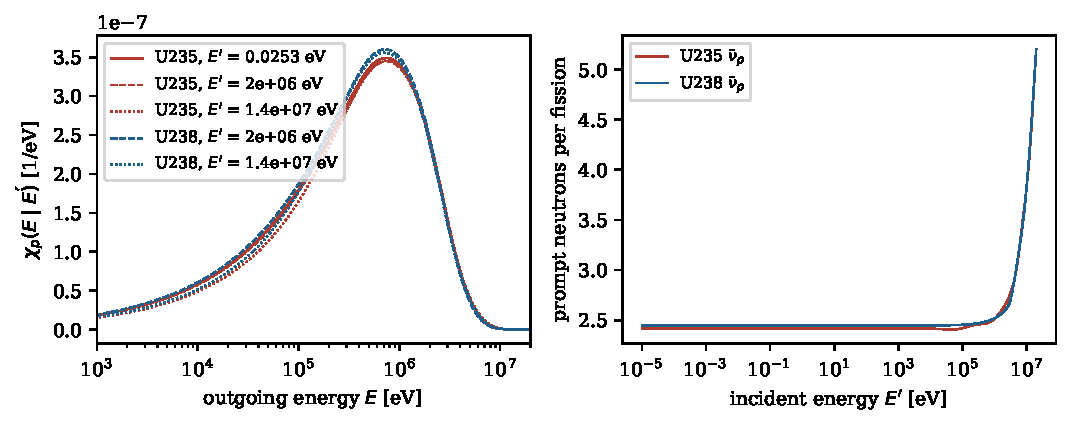
\includegraphics[width=\textwidth]{figures/nd_fission.pdf}
\caption{Left: prompt fission spectra of U-235 and U-238 at several incident energies: nearly the
same shape, peaked near 1 MeV, harder at high incident energy. Right: prompt $\bar\nu$ against incident
energy: flat below 1 MeV, rising linearly above, with steps at the second-chance threshold.}\label{fig:nd:fission}
\end{figure}

\section{How the data shape a reactor spectrum}\label{sec:nd:physics}

\subsection{Slowing down}

Fission neutrons are born near 2 MeV and are absorbed mostly below 1 eV, so they must lose six to
eight decades of energy. Elastic scattering off a nucleus at rest of mass ratio $A$ leaves a fraction
of the energy between $\alpha=((A-1)/(A+1))^2$ and 1; for isotropic CM scattering the ratio $E/E'$
is uniform on $[\alpha,1]$ (Figure~\ref{fig:nd:elastic}). The average lethargy gain per collision is
\begin{equation}
\xi=1+\frac{\alpha\ln\alpha}{1-\alpha}\approx\frac{2}{A+2/3},
\end{equation}
1 for hydrogen, 0.158 for carbon, 0.0084 for U-238: a neutron needs about 20 collisions in water
($\xi\approx0.92$) and 115 in graphite to slow from 2 MeV to thermal energies. In an infinite medium with constant scattering and no
absorption, the flux between the source and thermal energies is $\phi(E)\propto1/(\xi\Sigma_sE)$:
flat per unit lethargy, the $1/E$ spectrum visible in Figure~\ref{fig:nd:spectrum}.

\begin{figure}[t]\centering
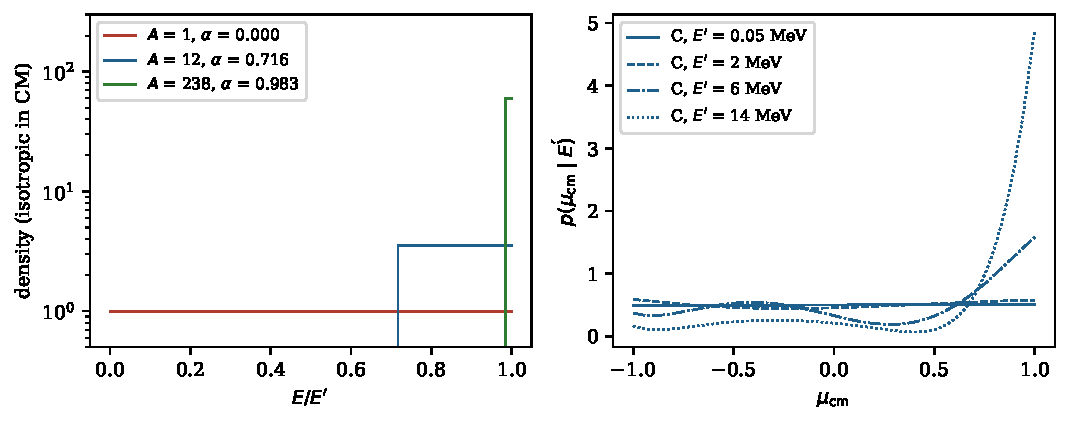
\includegraphics[width=\textwidth]{figures/nd_elastic.pdf}
\caption{Left: energy after one elastic collision with isotropic CM scattering, for $A=1$, 12 and
238. Right: CM angular distribution of elastic scattering on carbon: isotropic at 100 keV,
increasingly forward-peaked at MeV energies. Forward-peaked scattering is what the P$_0$ MG control
cannot represent.}\label{fig:nd:elastic}
\end{figure}

\begin{figure}[t]\centering
\begin{tikzpicture}[xscale=1.25]
\draw[->] (0,0) -- (10.5,0) node[right] {$\ln(E_0/E)$ (lethargy)};
\foreach \x/\l in {0/2 MeV,2/100 keV,5/100 eV,8/0.1 eV,10/0.01 eV} {\draw (\x,0.1)--(\x,-0.1) node[below,font=\scriptsize] {\l};}
\fill[accred!15] (0,0.2) rectangle (1.6,1.6); \node[note] at (0.8,1.85) {fission\\ source};
\fill[accorange!15] (1.6,0.2) rectangle (3,1.6); \node[note] at (2.3,1.85) {inelastic,\\ fast fission};
\fill[headblue!10] (3,0.2) rectangle (7.6,1.6); \node[note] at (5.3,1.85) {slowing down: $\phi\propto1/E$,\\ resonance absorption};
\fill[accgreen!15] (7.6,0.2) rectangle (10,1.6); \node[note] at (8.8,1.85) {thermal:\\ Maxwellian};
\foreach \x in {3.6,4.3,4.9,5.6,6.1,6.8} \draw[thick,accred] (\x,0.2) -- (\x,1.1);
\draw[-{Stealth},thick] (0.4,0.6) -- (1.1,0.6) -- (1.5,0.6) -- (2.2,0.6) -- (2.6,0.6);
\foreach \x in {3.1,3.5,3.9,4.3,4.7,5.1,5.5,5.9,6.3,6.7,7.1,7.5} \draw[-{Stealth},gray] (\x,0.45) -- ++(0.32,0);
\node[note] at (5.3,0.3) {graphite: $\xi=0.158$, about 115 collisions to thermal};
\end{tikzpicture}
\caption{The life of a neutron in lethargy. Fission emits at MeV energies; inelastic scattering and fast
fission act above 100 keV; elastic collisions move the neutron through the resonance range in steps of
$\xi$, where U-238 resonances (red) absorb; below about 1 eV the neutron thermalizes.}\label{fig:nd:cascade}
\end{figure}

\subsection{Resonance absorption and self-shielding}

As neutrons slow down past the U-238 resonances, the flux in the fuel dips sharply at each resonance:
the fuel absorbs so strongly at the resonance energy that the interior of the pin sees fewer neutrons
(\emph{spatial self-shielding}), and the flux depression in energy reduces the effective capture
(\emph{energy self-shielding}). Figure~\ref{fig:nd:resonances} shows both: the fuel's flux falls at
each resonance, and the graphite's falls too, since fewer neutrons at those energies leave the
fuel. A multigroup model must average these dips into a group constant; the averaging is done with a
weighting spectrum that is right only for the problem it came from. This is the dominant source of
the MG field's error and therefore of the residual (Section~\ref{sec:res:controlled}).

\begin{figure}[t]\centering
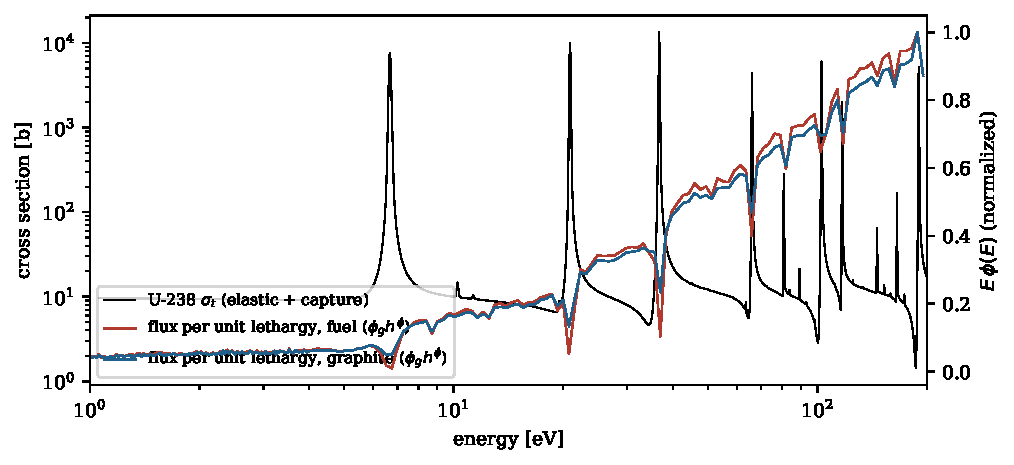
\includegraphics[width=\textwidth]{figures/nd_resonances.pdf}
\caption{U-238 resonances and the flux per unit lethargy in the fuel and graphite of the pincell
(from the CE lift tallies). The flux dips at every resonance; the group boundaries of CASMO-8 lie at
4 eV and 5.53 keV, so a single group must average across all of these structures.}\label{fig:nd:resonances}
\end{figure}

\subsection{Thermalization}

Below about 1 eV the neutron's energy is comparable to the target's thermal motion, so collisions can
\emph{raise} the energy. The flux tends to a Maxwellian
$\phi(E)\propto E\,e^{-E/kT}$, hardened by absorption. Free-atom (free-gas) scattering treats the
target as a gas at temperature $T$; chemical binding (S($\alpha,\beta$)) changes the exchange
of energy, most strongly for hydrogen in water and for graphite.

\begin{figure}[t]\centering
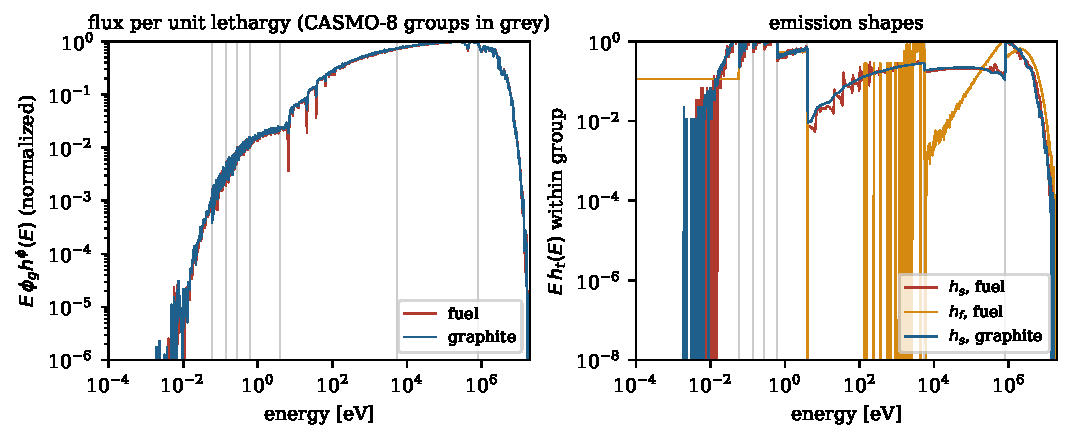
\includegraphics[width=\textwidth]{figures/nd_spectrum_lifts.pdf}
\caption{The graphite pincell's spectrum. Left: flux per unit lethargy in fuel and graphite, showing
the fission source above 100 keV, the $1/E$ slowing-down plateau with resonance dips, and the thermal
range. Right: the emission shapes the lifts carry within each group.}\label{fig:nd:spectrum}
\end{figure}

\begin{figure}[t]\centering
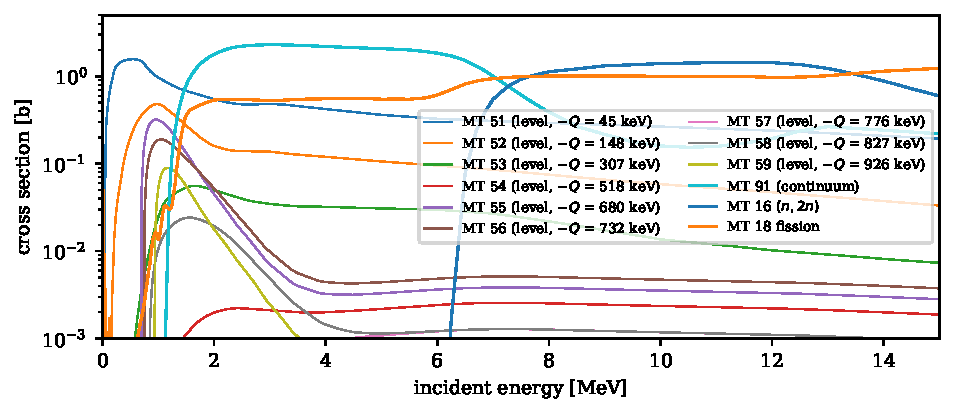
\includegraphics[width=\textwidth]{figures/nd_inelastic.pdf}
\caption{U-238 inelastic scattering to discrete levels (thresholds at 45, 148, \dots\ keV),
continuum, $(n,2n)$ and fission. Inelastic scattering moves neutrons from MeV to tens of keV in one
collision.}\label{fig:nd:inelastic}
\end{figure}

\section{How OpenMC samples each reaction}\label{sec:nd:openmc}

\subsection{The collision}

OpenMC's \code{collision()} (in \code{src/physics.cpp}) is entered at a collision site with the
particle's macroscopic and microscopic cross sections already computed by
\code{Material::calculate\_xs} at the particle's energy and temperature (with probability tables,
S($\alpha,\beta$) and multipole data where enabled). It proceeds:

\begin{algorithm}[h]
\caption{OpenMC's analog neutron collision (simplified)}
\DontPrintSemicolon
choose nuclide $m$ with probability $N_m\sigma_{t,m}/\Sigma_t$ \tcp*{\code{sample\_nuclide}}
\eIf{$\xi<\sigma_{s,m}/\sigma_{t,m}$}{scatter: \code{scatter(p, m)}}{
  absorption: create fission sites with expected count $w\,\nu\sigma_f/(k\,\sigma_t)$ (eigenvalue)\;
  survival biasing or analog kill\;
}
\end{algorithm}

\code{scatter()} chooses between elastic (with S($\alpha,\beta$) below its cutoff) and the other
scattering reactions by their cross sections, then calls:
\begin{itemize}
\item \textbf{\code{elastic\_scatter}}: samples a target velocity (\code{sample\_target\_velocity}):
  at rest if $A>1$ and $E\ge$ \code{free\_gas\_threshold}$\cdot kT$ (and the nuclide is not a
  resonant scatterer); otherwise a free-gas Maxwellian with the constant-cross-section approximation,
  or DBRC/RVS for resonant scatterers. It transforms to the CM frame, samples $\mu_{cm}$ from the
  angular distribution, rotates and transforms back.
\item \textbf{\code{sab\_scatter}}: samples from the S($\alpha,\beta$) tables (coherent elastic: a
  Bragg edge, then the cosine it implies; incoherent: discrete or continuous tables).
\item \textbf{\code{inelastic\_scatter}}: samples the product's distribution (\code{ReactionProduct::sample}),
  converts CM to lab where needed, and handles the yield: a fractional yield multiplies the weight,
  an integer yield $\nu>1$ banks $\nu-1$ copies with the \emph{same} outgoing state.
\end{itemize}
Fission (\code{create\_fission\_sites}) samples the reaction among partial fission reactions by
cross section (\code{sample\_fission}) and each neutron with \code{sample\_fission\_neutron}: prompt
or delayed by $\bar\nu_d/\bar\nu$, the delayed group by its yield, then the energy from the
corresponding distribution, resampled until $E<E_{max}$ of the data; isotropic direction.

\subsection{The sampling algorithms of the energy laws}

\begin{algorithm}[h]
\caption{Continuous tabular energy law (ENDF law 4 / ACE law 4), as in OpenMC}\label{alg:law4}
\DontPrintSemicolon
find $\ell$ with $E'_\ell\le E'<E'_{\ell+1}$; $r\gets(E'-E'_\ell)/(E'_{\ell+1}-E'_\ell)$ (log-log in some data)\;
$i\gets\ell+1$ with probability $r$, else $i\gets\ell$ \tcp*{stochastic interpolation}
sample $\hat E$ from table $i$ (histogram or linear-linear CDF inversion; discrete lines first)\;
$E_{lo}\gets(1-r)E^{(\ell)}_{min}+rE^{(\ell+1)}_{min}$;\quad $E_{hi}$ likewise\;
$E\gets E_{lo}+(\hat E-E^{(i)}_{min})\frac{E_{hi}-E_{lo}}{E^{(i)}_{max}-E^{(i)}_{min}}$\tcp*{unit-base rescaling}
\end{algorithm}

Its density is therefore a mixture of the two tables, each mapped onto the interpolated range with the
Jacobian $(E^{(i)}_{max}-E^{(i)}_{min})/(E_{hi}-E_{lo})$ (Section~\ref{sec:nd:openmc}). The other laws:
\begin{itemize}
\item \textbf{Maxwell} $f\propto\sqrt E\,e^{-E/\theta}$: sampled as $-\theta(\ln\xi_1+\ln\xi_2\cos^2(\pi\xi_3/2))$
  and rejected until $E\le E'-U$; its density is the Maxwellian renormalized to $[0,E'-U]$.
\item \textbf{Watt} $f\propto e^{-E/a}\sinh\sqrt{bE}$: sampled from a Maxwellian of temperature $a$ and a
  shift, $E=w+\frac{a^2b}{4}+(2\xi-1)\sqrt{a^2bw}$, with rejection on $[0,E'-U]$.
\item \textbf{Evaporation} $f\propto E\,e^{-E/\theta}$: by inversion of a gamma distribution, rejected on
  $[0,E'-U]$.
\item \textbf{Kalbach--Mann}: $E$ from law-4-like tables with tabulated precompound fraction $r$; then
  $\mu$ from $\frac{a}{2\sinh a}(\cosh a\mu+r\sinh a\mu)$ by a two-branch inversion.
\end{itemize}

\subsection{Free-gas elastic scattering in OpenMC}

Below the free-gas threshold (or for resonant scatterers), OpenMC samples a target velocity from the
distribution $P(\mathbf V)\propto|\mathbf v-\mathbf V|\,\sigma(|\mathbf v-\mathbf V|)\,M(\mathbf V)$, with
$M$ the Maxwellian at the material temperature. With constant $\sigma$ this is done by sampling the
target speed from a mixture of $V^3e^{-\beta V^2}$ and $V^2e^{-\beta V^2}$ and the cosine between target and
neutron with rejection on the relative speed. The neutron then scatters isotropically (or with the
tabulated CM distribution) in the CM frame of the pair. The exact density of this procedure is the
free-gas kernel above; the DBRC and RVS options for resonant scatterers replace the constant cross
section by the 0 K resonant one in the rejection step.

\begin{figure}[t]\centering
\begin{tikzpicture}[node distance=5mm and 8mm, every node/.style={font=\footnotesize}]
\node[box] (c) {collision at $(\vr,E,\vO)$\\ \code{calculate\_xs} done};
\node[box,below=of c] (nuc) {nuclide $m$ $\propto N_m\sigma_{t,m}$};
\node[box,below left=6mm and 6mm of nuc] (sc) {scatter: \code{scatter(p,m)}};
\node[box,below right=6mm and 6mm of nuc] (ab) {absorb: fission sites\\ $w\nu\sigma_f/(k\sigma_t)$, then kill\\ or survival biasing};
\node[box,below left=6mm and -10mm of sc] (el) {elastic\\ target velocity:\\ at rest / free gas};
\node[box,right=4mm of el] (sab) {S($\alpha,\beta$)\\ tables};
\node[box,right=4mm of sab] (inel) {inelastic, $(n,xn)$\\ product laws,\\ yield copies};
\node[box,below=8mm of ab] (fis) {\code{sample\_fission\_neutron}:\\ prompt/delayed, $\chi$, isotropic};
\draw[arr] (c)--(nuc); \draw[arr] (nuc)--(sc); \draw[arr] (nuc)--(ab);
\draw[arr] (sc)--(el); \draw[arr] (sc)--(sab); \draw[arr] (sc)--(inel); \draw[arr] (ab)--(fis);
\end{tikzpicture}
\caption{OpenMC's analog neutron collision and the routines this method reuses: the sampler route and
the flights call \code{scatter} and \code{sample\_fission\_neutron} on scratch particles.}\label{fig:nd:collision}
\end{figure}

\subsection{What a sampler does that a density must match}

An evaluator is correct only if it is the density of \emph{exactly} what the sampler does. Three
details matter in practice:
\begin{enumerate}
\item \textbf{Stochastic interpolation between incident tables.} For law 4, OpenMC picks table
  $\ell$ or $\ell+1$ with probability $1-r$ and $r$ and then rescales the outgoing energy to
  interpolated endpoints. The density is therefore a mixture of two rescaled tabulated densities,
  each with its Jacobian:
  $f(E\mid E')=(1-r)f_\ell(E_\ell(E))\frac{\dd E_\ell}{\dd E}+rf_{\ell+1}(E_{\ell+1}(E))\frac{\dd E_{\ell+1}}{\dd E}$.
  Without the Jacobian the density is wrong between grid points and right at them.
\item \textbf{Rejection on $E_{max}$} conditions the distribution; the density is renormalized
  accordingly.
\item \textbf{Target motion} below the free-gas threshold turns the elastic kernel from a curve in
  $(E,\mu_0)$ into a two-dimensional density; the stationary image formula no longer applies.
\end{enumerate}

\section{Consequences for this method}\label{sec:nd:consequences}

\subsection{Which reactions have densities today}

\begin{table}[t]\centering\small
\begin{tabularx}{\textwidth}{>{\raggedright}p{3.3cm}>{\raggedright}p{3.6cm}>{\raggedright}p{2.1cm}X}
\toprule
Reaction & OpenMC sampler & Route now & A density from the evaluation\\
\midrule
elastic, stationary target ($A>1$) & CM angle, two-body & evaluator & image formula \eqref{eq:elastic_image} (done)\\
fission, prompt and delayed & law 4 / Maxwell / Watt / evaporation & evaluator & density of the sampler incl.\ interpolation (done)\\
elastic, free gas (H, below threshold) & Maxwellian target & sampler & closed-form free-gas kernel (constant $\sigma$)\\
inelastic to a level (MT 51--90) & CM angle, two-body with $Q$ & sampler & image formula with $Q$: $E'$ from $(E,\mu_0)$, Jacobian\\
continuum (MT 91), law 4 & tabulated & sampler & as fission's law 4 (with angle)\\
Kalbach--Mann (law 44) & tabulated $E$, closed-form $\mu$ & sampler & product of law-4 density and the Kalbach angle density\\
law 61 & tabulated $E$, tabulated $\mu$ & sampler & interpolated tables, same Jacobians\\
$(n,xn)$ & as above, yield & sampler & as above, times the yield\\
S($\alpha,\beta$) incoherent inelastic & discrete or continuous tables & sampler & continuous: interpolation; discrete: mixture of points, not a density\\
S($\alpha,\beta$) coherent elastic & Bragg edges & sampler & discrete cosines: delta functions in $\mu$; an image formula in $E'$ per edge\\
unresolved resonances & probability tables & (off) & $\Sigma_t$ random per particle: $\E e^{-\tau}\ne e^{-\E\tau}$\\
\bottomrule
\end{tabularx}
\caption{Reactions, how OpenMC samples them, their route in this method, and how a density for the
evaluator route could be built from the evaluation.}\label{tab:nd:routes}
\end{table}

Table~\ref{tab:nd:routes} summarizes. Two things decide whether a density is worth building:
\begin{itemize}
\item \textbf{Variance.} An evaluator places the production at the destination's state, where the
  low term cancels it pointwise. On the sampler route the production lands elsewhere, and the low
  term must be cancelled by netting or pooling. The controlled residual study shows that for elastic
  scattering in graphite the density route is 7--10 times more efficient even after the low term is
  made exact; for fission, the sampler route with an exact low term is 5--10 times more efficient.
\item \textbf{Cost.} An evaluator costs a density evaluation per image; images multiply with the
  number of nuclides ($n_E$ grows), while the sampler costs one collision per incident energy.
\end{itemize}

\subsection{Densities from the evaluation, concretely}

\textbf{Discrete inelastic levels} are two-body reactions with $Q<0$. With the same notation as
elastic, the lab outgoing energy is $E=E'\gamma(\mu_0;E',Q)$, now depending on $E'$ through the
threshold factor $\Delta=\sqrt{1+(A+1)Q/(AE')}$; for each $(E,\mu_0)$ there are at most two images
$E'$, found by a one-dimensional root solve, with Jacobian $|\partial E/\partial E'|^{-1}$. The CM
angular density comes from MF 4 exactly as for elastic.

\textbf{Continuum and correlated laws} already have the structure of densities: law 4 tables are
densities in $E$ at each incident grid point; Kalbach--Mann's angular part is closed-form; law 61
tabulates $p(\mu\mid E,E')$. The work is to reproduce OpenMC's interpolation and frame transformation
exactly, as was done for fission.

\textbf{Free-gas elastic scattering} with a constant cross section has a closed-form
double-differential kernel. In the ENDF convention, with $\alpha=(E+E'-2\mu_0\sqrt{EE'})/(AkT)$ and
$\beta=(E-E')/kT$,
\begin{equation}
\frac{\dd^2\sigma}{\dd E\,\dd\mu_0}(E'\to E,\mu_0)=\frac{\sigma_b}{2kT}\sqrt{\frac{E}{E'}}\,S(\alpha,\beta),
\qquad S(\alpha,\beta)=\frac{1}{\sqrt{4\pi\alpha}}\exp\!\Big(-\frac{(\alpha+\beta)^2}{4\alpha}\Big),
\end{equation}
with $\sigma_b=\sigma_{free}(A+1)^2/A^2$ the bound-atom cross section. It is a genuine
two-dimensional density, so the energy integral no longer collapses onto an image: an incident energy
must be drawn, as for fission. (OpenMC's free-gas sampler with constant $\sigma$ samples exactly this
kernel.)

\textbf{S($\alpha,\beta$)} continuous incoherent inelastic tables are densities by interpolation;
discrete tables (equally probable cosines and energies) are not, and coherent elastic is a set of
delta functions in $\mu$, which can be handled like elastic images (one $E'$ per Bragg edge and
$\mu_0$).

\subsection{What stays on the sampler route}

Reactions whose densities are not worth building (small production, discrete tables) stay on the
sampler route and are made exact by the registry: they are estimated by OpenMC's own routines, so
every law OpenMC supports is supported. Their cost is variance, and the low term they cannot cancel
pointwise is handled by the exact low term in the netting bins.
